\chapter{Návrh řídícího systému}
Jak bylo zmíněno výše, vstupy do regulátoru jsou statorový proud v $dq$ souřadnicích $i_{s_{dq13}}$, otáčky motoru $\omega_m$ a generovaný moment $T$. Na obrázku \ref{fig:regulator blokac} je blokové schéma navrhovaného regulátoru.

Jedná se o kaskádní řízení obsahující proudovou a rychlostní smyčku. Rychlostní regulátor na základě rozdílu mezi požadovanou a měřenou rychlostí generuje požadovaný moment $T^*$. Pro požadovaný moment je potom generován odpovídající vektor proudu $i_{dq_{13}}$. Následuje proudový regulátor, jehož výstupem je požadované napětí $V^*_{dq_13}$, to je transformováno na $V_{\alpha \beta_{1,3}}$, které je vstupem do modulátoru popsaného výše. V této kapitole jsou postupně představeny a podrobně rozebrány jednotlivé bloky regulační smyčky. 

\begin{figure}[h]
\centering
\resizebox{\textwidth}{!}{
\begin{tikzpicture}[
    block/.style = {draw, rectangle, minimum height=3cm, minimum width=3.4cm, align=center},
    arrow/.style = {->, thick},
    node distance=2.1cm
]

    % Bloky
    \node (wref) {$\omega_m^{*}$};
    \node[block, right=of wref] (torque_ctrl) {Regulátor\\ momentu};
    \node[block, right=of torque_ctrl] (current_ref) {Generátor\\ referenčního proudu};
    \node[block, right=of current_ref] (current_ctrl) {Proudový\\ regulátor};
    \node[block, right=of current_ctrl] (dq2ab) {$dq \rightarrow \alpha\beta_{1,3}$};
    \node[block, right=of dq2ab] (mod) {Modulátor a\\ Pohon};
    \node[block, below=of dq2ab] (todq) {$abcd \rightarrow dq$};
    
    % Měřené signály
    \node[below=1.2cm of torque_ctrl] (wmeas) {$\omega_m$};
    \node[below=1.2cm of current_ctrl] (imeas) {$i_{s\,dq13}$};
    
    % Spojení s popisky
    \draw[arrow] (wref) -- (torque_ctrl);
    
    \draw[arrow] (wmeas) -- (torque_ctrl);
    
    \draw[arrow] (torque_ctrl) -- 
        node[midway, above] {$T^{*}$}
        (current_ref);
    
    \draw[arrow] (current_ref) -- 
        node[midway, above] {$i^{*}_{dq13}$}
        (current_ctrl);
    
    \draw[arrow] (imeas) -- (current_ctrl);
    
    \draw[arrow] (current_ctrl) -- 
        node[midway, above] {$V^{*}_{dq13}$}
        (dq2ab);
    
    \draw[-stealth] (dq2ab) -- 
        node[midway, above] {$V^{*}_{\alpha\beta_{1,3}}$}
        (mod);
    \draw[<-]  (todq.east)  -|(mod.south) ;
    \draw[->] (todq)  -| (imeas.south);
    \draw[->] (todq)  -| (wmeas.south);
    
\end{tikzpicture}}
\caption{Blokové schéma navrhovaného regulátoru}
\label{fig:regulator blokac}
\end{figure}



\section{Proudová smyčka}
Cílem regulátoru je udržovat vektor proudu na požadované hodnotě, problém je rozdělen na regulaci proudu v jednotlivých souřadnicích zvlášť. Příspěvek od ostatních složek je buď kompenzován pomocí substituce, nebo považován za poruchu a je kompenzován I složkou regulátoru. V kapitole jsou představeny a porovnány oba přístupy.

\subsubsection{Odstranění křížové vazby}
Přepsáním rovnice \ref{eq:model dq v final} získám diferenciální rovnici \ref{eq:ss idq s kriz} popisující proud motoru, problematický pro regulaci je člen  $- \omega_e(t) \left( Li(t) + \gamma \Psi\right)$,  reprezentující zpětné elektromotorické napětí. To je problematické protože je závislé na otáčkách motoru $w$ a zároveň matice E není diagonální uzpůsobuje tedy křížovou vazbu mezi jinak nezávislými systémy. 

\begin{equation}
    \label{eq:ss idq s kriz}
     \frac{di}{dt} = \frac{1}{L_s} \left( v_{dq_{13}} - R_s i_{dq_{13}} - \omega_{fr}E \left( L_{s}i_{dq_{13}} + \gamma \Psi_{PM}\right) \right)
\end{equation}



Nechtěný člen eliminuji zavedením substituce za $v$ (\ref{eq:substituce v}). Substituovaný výraz je závislý na rychlosti rotace elektrického pole, tu lze spočítat z měřených otáček motoru jako $\omega_e=\omega_m \cdot p $, a proudu statorem, který přímo měřím. Dosazením do rovnice \ref{eq:ss idq s kriz} získávám systém popsaný \ref{eq:proud bez krize}, jedná se o 4 nezávislé SISO systémy prvního řádu. Pro ně stačí navrhnout 4 jednoduché regulátory.  


\begin{equation}
\label{eq:substituce v}
    v(t)=u(t) +  \omega(t) E \left(  i(t) + \gamma \Psi\right)
\end{equation}

\begin{equation}
    \label{eq:proud bez krize}
     \frac{di}{dt} = \frac{1}{L_s} \left( u_{dq_{13}} - R_s i_{dq_{13}}  \right)
\end{equation}

Při běžném provozu lze výraz kompenzovat i I složkou regulátoru, nicméně při rychlých změnách dosahuje regulátor s kompenzací lepších výsledků.

\subsubsection{Návrh PI regulátoru}
Vzhledem k tomu, že se jedná o soustavu 1. řádu, volím PI regulátor s přenosovou funkcí:

\begin{equation}
    \label{eq:PI}
    C(p) = K_p \frac{1 + T_i p}{T_i p}
\end{equation}



Z rovnice \ref{eq:proud bez krize} lze pro každou z os odvodit přenosovou funkci soustavy:

\begin{equation}
    \label{eq:tf proud}
    G(p) = \frac{1}{R_s + L_s p}
\end{equation}

Nulu regulátoru umístím tak, aby kompenzovala pól soustavy, tedy $T_i = L_s / R_s$.Zesílení $K_p$ jsem volil tak, aby omega řezu odpovídala ${1}/{\tau}$. Výsledný přenos regulátoru převedu do diskrétní podoby s periodou vzorkování $T_s$. Získané hodnoty jsem implementoval do regulátoru v Simulinku podle rovnice \ref{eq:PI diskretni} a manuálně doladil.

\begin{equation}
    \begin{gathered}
    T_i=\frac{L_s}{R_s}\\  %POZOR MOZNA *Ts
    K_p=T_i \cdot \omega_c \cdot R_s= \frac{L_s}{R_s} \cdot \frac{R_s}{L_s} \cdot R_s =R_s
    \end{gathered}
\end{equation}

\begin{equation}
    \label{eq:PI diskretni}
    F_R(z^{-1}) = K_d \left(1 + \frac{1}{T_d(1 - z^{-1})}\right)
\end{equation}


Na obrázku \ref{fig:bez a s cross} je vidět porovnání odezvy motoru na skokovou změnu proudu s a bez kompenzací zpětného elektromotorického napětí. Je vidět, že regulátor s kompenzací má výrazně menší překmit a dříve se ustálí. Kompenzace je v tomto případě jednoduchá, neboť mám plnou kontrolu nad modelem motoru.

Pro reálný motor kompenzace nebude nikdy dokonalá, proto jsem regulátor i včetně všech nadřazených ladil na systému bez kompenzace a následně přidal kompenzaci, která zlepšila odezvu motoru zejména při rychlých změnách požadovaného proudu. 

\begin{figure}[!h]
    \centering
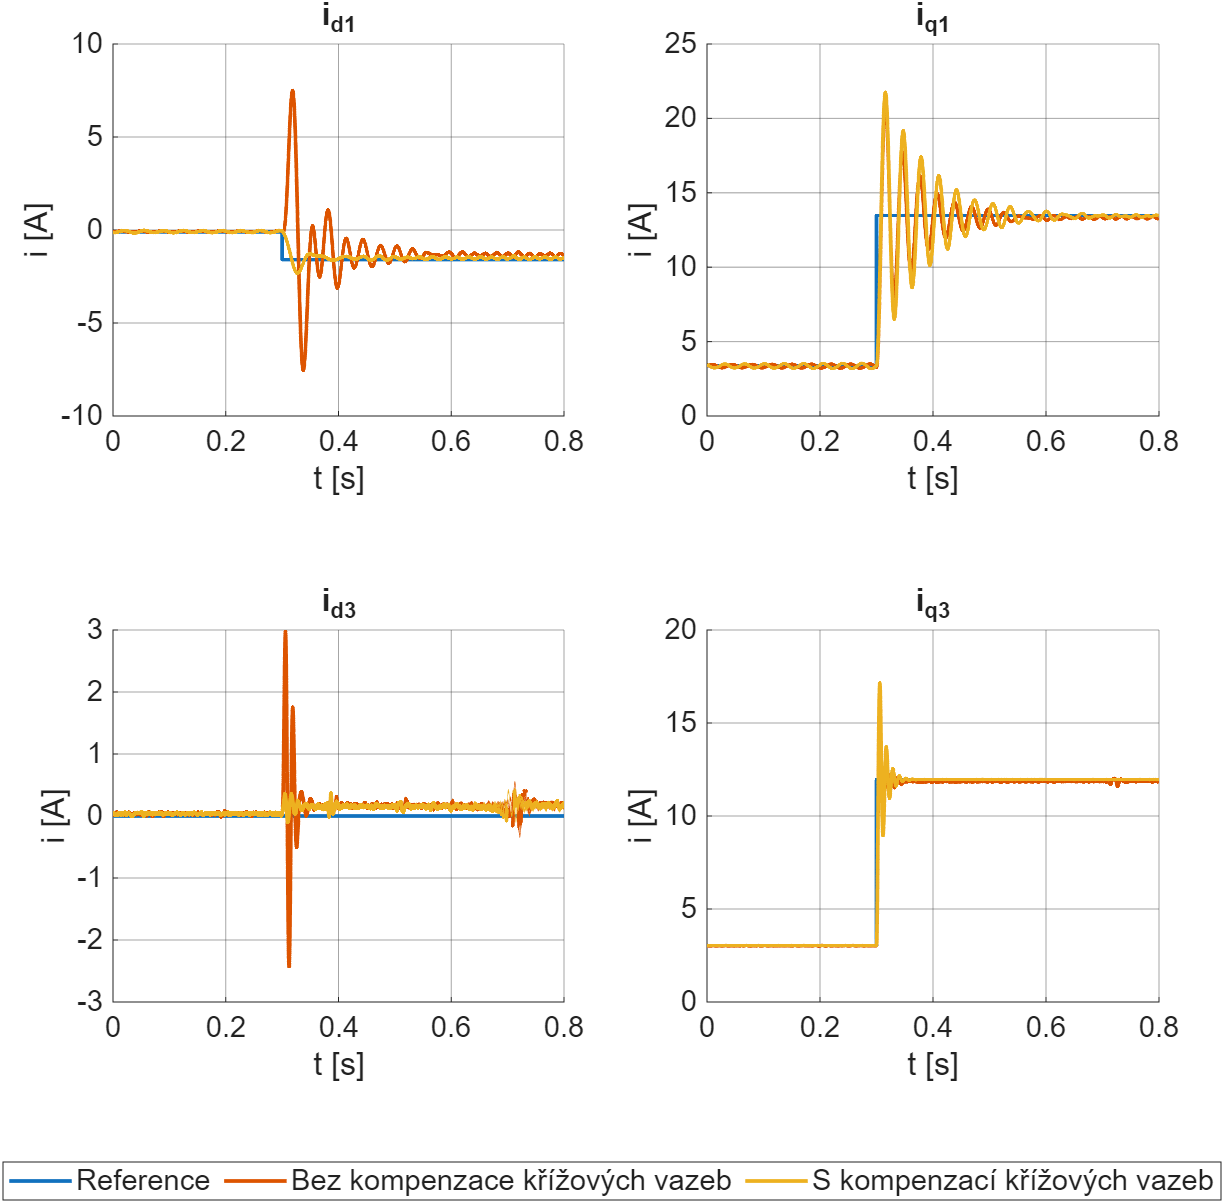
\includegraphics[width =\linewidth]{obrazky/cross_compens.png}
\caption{Porovnání regulace proudu s a bez kompenzace zpětného elektromotorického napětí}
\label{fig:bez a s cross}
\end{figure} 




\section{Řízení momentu}
\label{kap:MTPA}
Cílem tohoto bloku je pro požadovaný moment $T^*$, určený nadřazeným regulátorem rychlosti, vygenerovat požadovaný vektor proudů $i_{dq_{13}}^*$.


Moment generovaný motorem je dán rovnicí \ref{eq:moment dq} \cite{multiphasePMSM}. Pokud za jednotlivé komponenty $\psi_s$ dosadíme z rovnice \ref{eq:model dq flux final}, získáme po úpravě vztah \ref{eq:moment dq proud}, kde $p$ odpovídá počtu pólových dvojic. 
\begin{equation}
    \label{eq:moment dq}
    T_e = \frac{5}{2} p \cdot (\psi_{sd1} i_{q1} - \psi_{sq1} i_{d1} + 3 \psi_{sd3} i_{q3} - 3 \psi_{sq3} i_{d3}) 
\end{equation}


  \begin{equation}
     \label{eq:moment dq proud}
      T_e = \frac{5}{2} p \cdot \left[
     \left(\Psi _{\mathrm{PM}}+i_{\mathrm{d1}}\,\left(L_{\mathrm{d1}}-L_{\mathrm{q1}}\right)\right)\,i_{\mathrm{q1}}+
     \left(3\,L_{\mathrm{d3}}-3\,L_{\mathrm{q3}}\right)\,i_{\mathrm{q3}}\cdot i_{\mathrm{d3}} \right]
 \end{equation}
 Jelikož $L_{d3}=L_{q3}=Ls$ získáme finální vztah pro moment \ref{eq:moment dq proud final}, ten je nezávislý na $i_{dq_3}$.

 \begin{equation}
     \label{eq:moment dq proud final}
     T_e = \frac{5}{2} p \cdot 
     \left(\Psi _{\mathrm{PM}}+i_{\mathrm{d1}}\,\left(L_{\mathrm{d1}}-L_{\mathrm{q1}} \right) \right)i_{\mathrm{q1}}
 \end{equation}

Moment je tedy přímo možné ovlivnit proudem první harmonické $i_{dq_1}$. Jelikož $q1$ složka indukčnosti bývá větší než $L_{d1}$, je výraz $\left(L_{\mathrm{d1}}-L_{\mathrm{q1}} \right) $ záporný\cite{petros}.

Nejjednodušším přístupem k regulaci momentu je nastavit referenci $i_{d1}^*=0$ a moment regulovat přímo pomocí $i_{q1}$. Toto řešení je dostatečně robustní a jednoduché na implementaci i na ladění. Nevýhodou tohoto řešení je, že tím dochází ke snížení maximálního možného generovaného momentu. 

Moment jde ještě zvýšit aplikováním záporného proudu $i_{d1}$. Pro požadovaný moment potom existuje vztah mezi $i_{d1}$ a $i_{q1}$, kterým jde daného momentu dosáhnout.


Pro zvolení dvojice proudů lze použít například MTPA (maximum torque per ampere) tedy maximální moment na ampér. Algoritmus spočívá v tom že pro daný moment vybere takovouto dvojici proudů aby byl maximalizován moment generovaný jedním ampérem dodaným do motoru.\cite{petros}





\subsection{Injekce 3.harmonické}
Model motoru v Matlabu popsaný v kapitole \ref{kap:model abcd} není přesný. Nezohledňuje vliv permanentního magnetu i v rovině $dq_3$. Rovnice \ref{eq:model dq flux final} tento jev nezohledňuje. Při zohlednění vlivu permanentního magnetu na 3.~harmonickou složku statorového indukčního toku odpovídá spíše rovnici \ref{eq:model dq flux 3}. Kde k je konstanta vyplývající z konstrukce motoru, pohybuje se většinou v rozmezí $0.2-0.3$. Tato změna $\gamma$ ovlivní i velikost momentu, rovnice \ref{eq:moment dq proud} pro nový popis neplatí, pokud vyjdu z rovnice \ref{eq:moment dq} tak po dosazení získám nový vztah pro moment \ref{eq:moment 3rd}, a z ní po úpravě \ref{eq:moment 3rd final}.
\begin{equation}
    \label{eq:model dq flux 3}
    \psi_{s_{dq}}=
    \underbrace{
     \begin{bmatrix}    
        L_{d1} &0&0&0\\
        0 &L_{q1}&0&0\\
        0 &0&L_{d3}&0\\
        0 &0&0&L_{q3}\\
    \end{bmatrix}}_{L_{s_{dq}}}
    \cdot i_{dq}+ 
    \underbrace{
    \begin{bmatrix}
        1 \\ 0 \\k \\0 
    \end{bmatrix}}_{\gamma_{dq}} \cdot \Psi_{PM}
\end{equation}


\begin{equation}
    \label{eq:moment 3rd}
         T_e = \frac{5}{2} p \cdot \left[
     \left(\Psi _{\mathrm{PM}}+i_{\mathrm{d1}}\,\left(L_{\mathrm{d1}}-L_{\mathrm{q1}}\right)\right)\,i_{\mathrm{q1}}+
     \left( k\cdot \Psi_{PM}+ i_{\mathrm{d3}} \left(L_{\mathrm{d3}}-\,L_{\mathrm{q3}}\right)\right)3\,i_{\mathrm{q3}}\right]
\end{equation}

\begin{equation}
    \label{eq:moment 3rd final}
       T_e = \frac{5}{2} p \cdot \left[
     \left(\Psi _{\mathrm{PM}}+i_{\mathrm{d1}}\,\left(L_{\mathrm{d1}}-L_{\mathrm{q1}}\right)\right)\,i_{\mathrm{q1}}+
     3\,k\cdot \Psi_{PM}\cdot\,i_{\mathrm{q3}}\right]
\end{equation}

Na rozdíl od předchozího modelu je generovaný moment nyní ovlivněn také 3.harmonickou složkou proudu. Pokud je proud $i_{q\,3}$ nenulová, motor schopný generovat oproti předchozímu přístupu větší moment. 



\subsection{Určení referenčního proudu}
K určení vektoru proudu pro požadovaný moment slouží lookup tabulka, která pro požadovaný moment $T^*$ přiřadí odpovídající vektor proudu $i_{dq_{13}}^*$.

Hodnoty jednotlivých proudů musí generovat odpovídající moment daný  rovnicí \ref{eq:moment 3rd final}. Cílem je zároveň minimalizovat tepelné ztráty v motoru dané jako $P_{loss} = I^2 \cdot R$, kde $I$ odpovídá celkové velikosti proudu dodaného do motoru. Odpor vinutí $R$ je konstanta a polohu minima neovlivňuje, cílem je tedy minimalizovat druhou mocninu celkového proudu. Dostávám nákladovou funkci $J$ (rovnice \ref{eq:optimalni proud}), kterou minimalizuji.

\begin{equation}
    \label{eq:optimalni proud}
    J_{min} = i_{d1}^2 + i_{q1}^2 + i_{d3}^2 + i_{q3}^2
\end{equation}

Zároveň je nutné dodržet omezující podmínky plynoucí z konstrukce střídače. Maximální velikost odebíraného proudu je limitována parametry DC zdroje hodnotou $I_{DC\text{max}}$ (podmínka \ref{eq:Idc max}).

\begin{equation}
    \label{eq:Idc max}
    \sqrt{i_{d1}^2 + i_{q1}^2 + i_{d3}^2 + i_{q3}^2} \leq I_{DC\text{max}}
\end{equation}

Dále je nutné zajistit, že nebude překročen maximální proud jednotlivými tranzistory každé z fází. Maximální proud tranzistorem označuji jako $i_{sw\text{-max}}$. Ten musí být větší než maximální okamžitý proud protékající jednou z fází, daný jako superpozice základní a třetí harmonické fázového proudu (rovnice \ref{eq:okamzity i}). V nejhorším případě, kdy je fázový posun mezi $\hat{I}_1$ a $\hat{I}_3$ nulový, dosahuje maximální okamžitý proud fází hodnoty dané rovnicí \ref{eq:isw max}. Dostávám tak druhou omezující podmínku \ref{eq:podm sw}.

\begin{equation}
    \label{eq:okamzity i}
    i_{n}(t) = \hat{I}_1 \cos(\omega_e t + \varphi_1) + \hat{I}_3 \cos(3\,\omega_e t + \varphi_3)
\end{equation}

\begin{equation}
    \label{eq:isw max}
    i_{n,\text{max}} = \hat{I}_1 + \hat{I}_3 = \sqrt{i_{d1}^2 + i_{q1}^2} + \sqrt{i_{d3}^2 + i_{q3}^2}
\end{equation}

\begin{equation}
    \label{eq:podm sw}
    \sqrt{i_{d1}^2 + i_{q1}^2} + \sqrt{i_{d3}^2 + i_{q3}^2} \leq i_{sw\text{-max}}
\end{equation}

%Podmínka \ref{eq:podm sw} je vždy silnější než podmínka \ref{eq:Idc max}, neboť z nerovnosti $\sqrt{A^2+B^2} \leq A + B$ (platné pro $A,\,B \geq 0$) plyne, že splnění podmínky \ref{eq:podm sw} automaticky zaručuje splnění podmínky \ref{eq:Idc max}. Podmínku \ref{eq:Idc max} proto lze z optimalizačního problému vypustit a uvažovat pouze podmínku \ref{eq:podm sw}.

Z rovnice \ref{eq:moment 3rd final}, nákladové funkce \ref{eq:optimalni proud} a podmínek \ref{eq:Idc max} a \ref{eq:podm sw} vyplývá optimalizační problém, který řeším v matlabu pomocí funkce \texttt{fmincon}. Pro každý požadovaný moment $T^*$ je optimalizační problém řešen a získávám odpovídající vektor proudu $i_{dq_{13}}^*$. Výsledné hodnoty jsou uloženy do lookup tabulky, která je využívána v reálném čase pro určení referenčního vektoru proudu pro daný požadovaný moment. Vypočítané optimální proudy v závislosti na požadovaném momentu jsou zobrazeny na grafu \ref{fig:matpa}. 

Pokud je proud generovaný bez injekce 3.~harmonické, maximální teoretický moment je 14,76~Nm, s injekcí 3.~harmonické je možné generovat až 17,88~Nm. Pro nejjednodušší přístup k regulaci momentu, kdy je pouze $i_{q1}$ nenulová, je maximální moment pouze 9,8~Nm.


\begin{figure}[!h]
     \centering
     % První obrázek
     \begin{subfigure}[b]{0.8\textwidth}
         \centering
         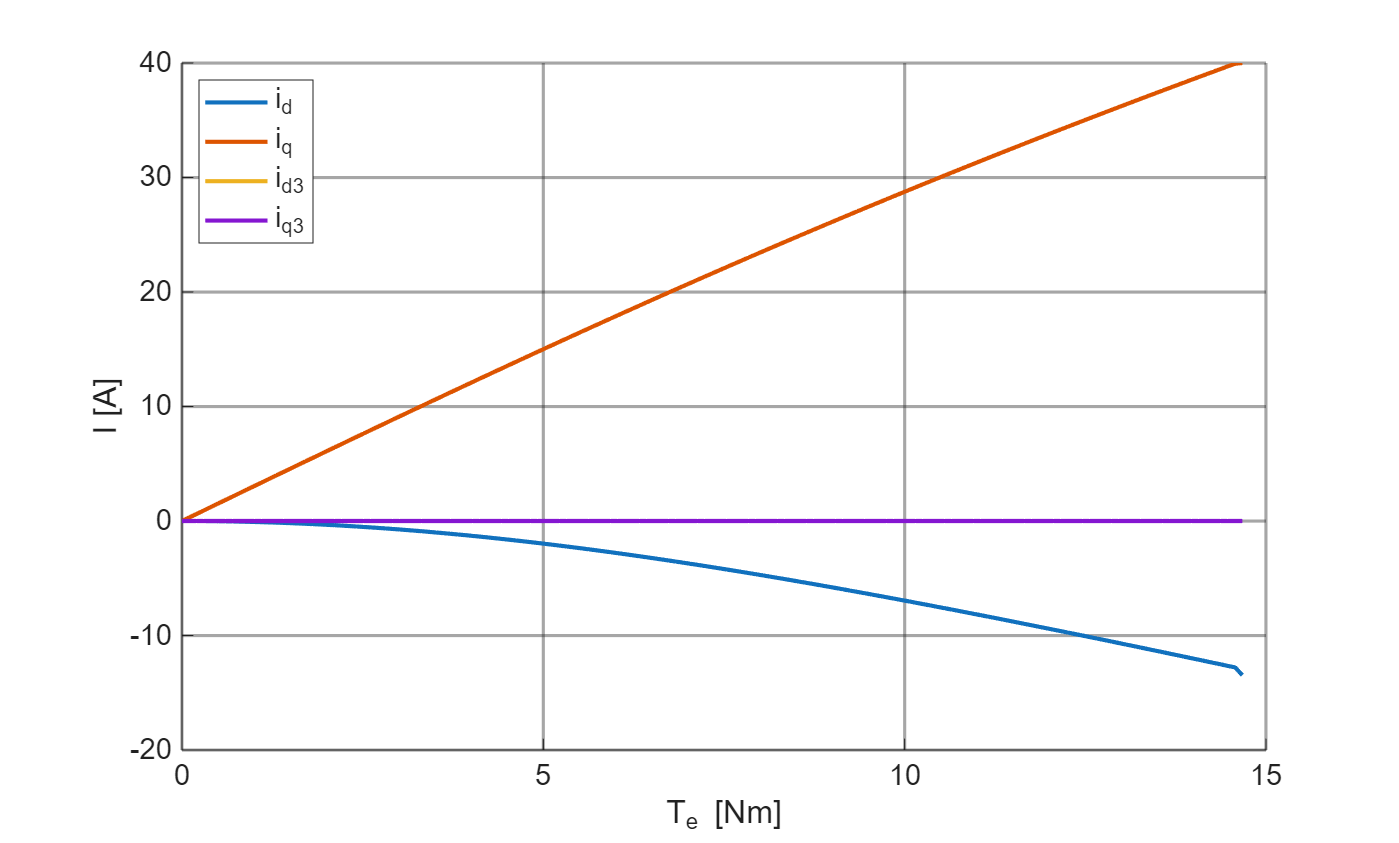
\includegraphics[width=\textwidth]{obrazky/MTPA1.png}
         \caption{Bez injekce 3.harmonické složky}
         \label{fig:mtpa 1}
     \end{subfigure}
     \hfill 
     % Druhý obrázek
     \begin{subfigure}[b]{0.8\textwidth}
         \centering
         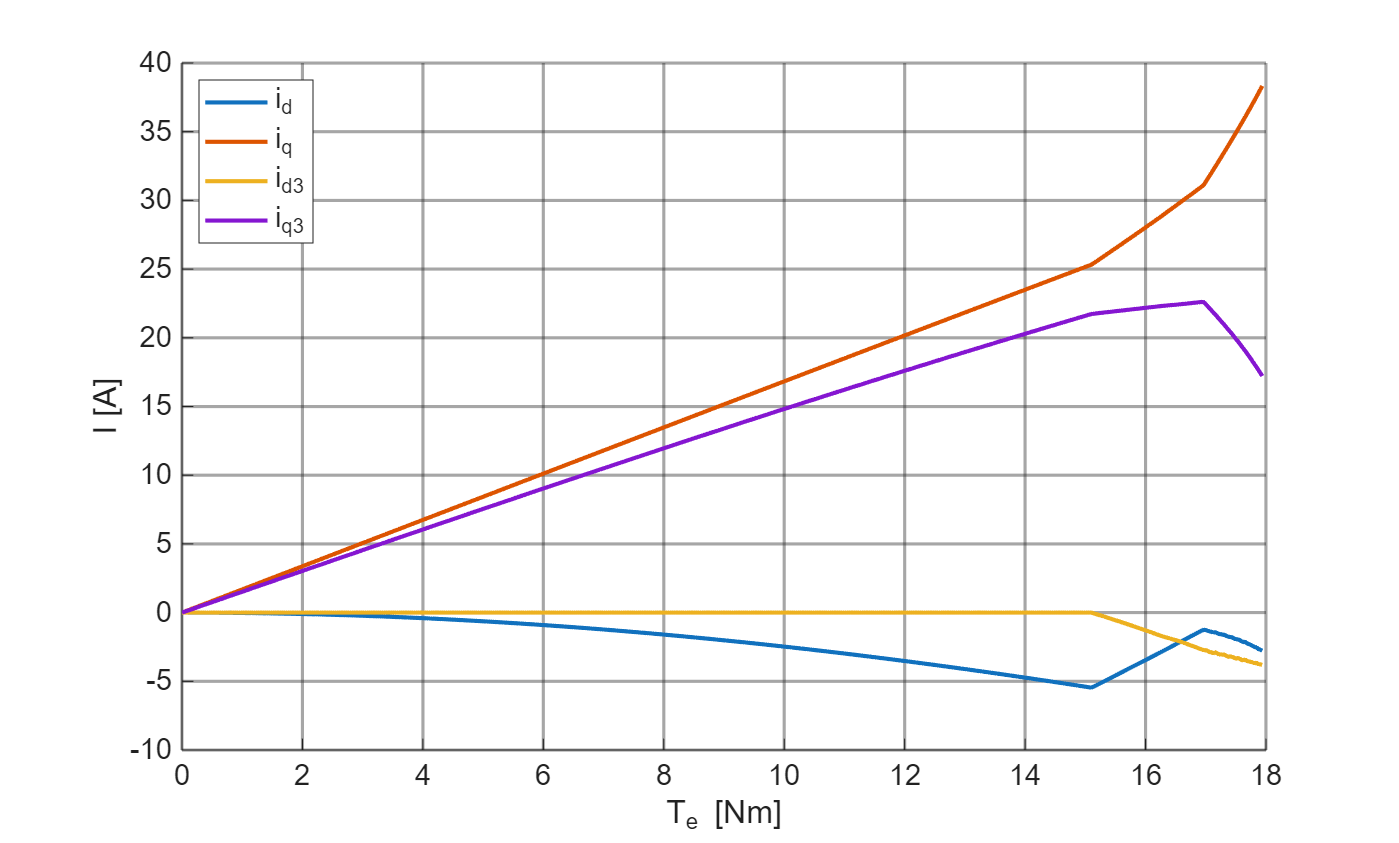
\includegraphics[width=\textwidth]{obrazky/MTPA3.png}
         \caption{S injekcí 3.harmonické složky}
         \label{fig:mtpa 3}
     \end{subfigure}
    \caption{Optimalizované proudy pro požadovaný moment}
    \label{fig:matpa}
\end{figure}

\subsubsection{Limity MTPA a jejich řešení}
Tato MTPA tabulka zajišťuje optimální využití proudu, ale je platná pouze pokud otáčky motoru nepřesahují definovanou mez $\omega_{base}$. Pro vyšší otáčky dochází k růstu zpětného elektromotorického napětí, které může překračovat napětí zdroje. Výstup proudového regulátoru je saturován na maximu, motor systém není schopen dosáhnout požadovaného proudu, tedy ani momentu. Řešením je oslabování magnetického pole aktivním potlačením magnetického toku $\psi_s$ v ose d1 a d3. Tím dojde ke snížení zpětně indukovaného napětí v ose q1, q3. Díky tomu je pohon schopen generovat proud a tím pádem i moment i při vyšších otáčkách.

Strategie pro určení referenčních proudů v této oblasti $\omega > \omega_{base}$ je podobná MTPA, jenom v téže situaci je hlavním cílem maximálně využít dostupné napětí \ref{eq:MTPV napeti}. Ostatní podmínky pro limit proudů \ref{eq:podm sw}, \ref{eq:isw max} a výpočet momentu zůstávají beze změny.

\begin{equation}
    \label{eq:MTPV napeti}
    \frac{1}{2} V_{dc}\geq \sqrt{V_d^2 +V_q^2}
\end{equation}
    

\begin{equation}
   \label{eq:MTPV cost f}
   J=\sqrt{(V_{d1}+V_{d3})^2 + (V_{q1}+V_{q3}^2)}
\end{equation}
Pokud tedy otáčky motoru přesáhnou $\omega_{base}$ určenou jako kladný kořen rovnice \ref{eq:omega base}, přejdu na generování referenčních proudů z MTPA strategie na MTPV \cite{fieldVeak}

\begin{equation}
    \label{eq:omega base}
    \omega_{base} = \frac{-b + \sqrt{b^2 - 4ac}}{2a}
\end{equation}

kde:

\begin{equation}
    \label{eq:omega base koef}
    \begin{aligned}
    a &= L_{q1}^2\,i_{q1}^2 + L_{d1}^2\,i_{d1}^2 + 9L_{q3}^2\,i_{q3}^2 + 9L_{d3}^2\,i_{d3}^2
        + \Psi_{PM}^2 + 9k^2\Psi_{PM}^2 \\
      &\quad + 2\Psi_{PM}\,i_{d1}\,L_{d1} + 18k\,\Psi_{PM}\,i_{d3}\,L_{d3} \\[4pt]
    b &= -2R_s\,i_{d1}\,L_{q1}\,i_{q1} + 2R_s\,i_{q1}\,L_{d1}\,i_{d1}
        + 2R_s\,i_{q1}\,\Psi_{PM} \\
      &\quad - 6R_s\,i_{d3}\,L_{q3}\,i_{q3} + 6R_s\,i_{q3}\,L_{d3}\,i_{d3}
        + 6R_s\,i_{q3}\,k\,\Psi_{PM} \\[4pt]
    c &= R_s^2\!\left(i_{q1}^2 + i_{d1}^2 + i_{q3}^2 + i_{d3}^2\right)
        - \left(\frac{V_{dc}}{2}\right)^{\!2}
    \end{aligned}
\end{equation}


V \cite{fieldVeak} je odvozeno, že optimální proud $i_{d1}$ vycházející z výše zmíněných předpokladů odpovídá, lze jej získat offsetem požadovaného proudu určeného MTPA o $i_{ds1}$ daný rovnicí \ref{eq:ids1 MTPV}.

\begin{equation}
    \label{eq:ids1 MTPV}
    i_{ds1} = \frac{-2L_{d1}\Psi_{PM} + \sqrt{4L_{d1}^2\Psi_{PM}^2 - 4\!\left(L_{d1}^2 - L_{q1}^2\right)\!\left(\Psi_{PM}^2 + L_{q1}^2\hat{I}_1^2 - \dfrac{V_{dc}^2}{4\omega_{fr}^2}\right)}}{2\!\left(L_{d1}^2 - L_{q1}^2\right)}
\end{equation}

Z ní lze potom dopočítat zbývající složky proudu $i_{qs1}$, $i_{qs3}$ a $i_{ds3}$ jako :

\begin{equation}
    \label{eq:iqs1 MTPV}
    i_{qs1} = \sqrt{\hat{I}_1^2 - i_{ds1}^2}
\end{equation}

\begin{equation}
    \label{eq:ids3 MTPV}
    i_{d3s} = k_3\sqrt{i_{ds1}^2 + i_{qs1}^2}\;\sin\!\left(3\arctan\!\left(\frac{i_{d1}}{i_{qs1}}\right)\right)
\end{equation}

\begin{equation}
    \label{eq:iqs3 MTPV}
    i_{qs3} = k_3\sqrt{i_{ds1}^2 + i_{qs1}^2}\;\cos\!\left(3\arctan\!\left(\frac{i_{sd1}}{i_{qs1}}\right)\right)
\end{equation}

Konstanta $k_3$ stanovuje poměr 1. a 3. harmonické. V článku je volena $k_3 = 0{,}15$ \cite{fieldVeak}. Tato metoda je výrazně závislá na přesných parametrech motoru.


\section{Regulace otáček}
Závislost otáček na momentu jak byla popsána v kapitole \ref{kap:mechanika} lze zapsat jako operátorový přenos \ref{eq:prenos mechaniky}. Pro návrh regulátoru jsem použil stejný přístup jako pro návrh proudových regulátorů. Tedy umístění nuly regulátoru tak, aby kompenzovala pól soustavy, a zesílení zajišťující frekvenci řezu odpovídající časové konstantě. Hodnoty jsem opět manuálně doladil.

\begin{equation}
    \label{eq:prenos mechaniky}
    G(p) = \frac{1}{Jp + b}
\end{equation}

Umístěním nuly regulátoru na pól soustavy a volbou zesílení pro požadovanou frekvenci řezu $\omega_c$ jsem získal vztahy:

\begin{equation}
    \label{eq:konstanty reg otacky}
    \begin{gathered}
        T_i = \frac{J}{b} \\
        K_p = J \cdot \omega_c= J \cdot \frac{b}{J}=b
    \end{gathered}
\end{equation}